\textcolor{red}{\section{Updated Experiments With RFNet on Finger Knuckle v3 Dataset}}

\textcolor{red}{Because in the previous experiments on the Finger Knuckle V3 Dataset, I used the segmented finger Knuckle of dataset. Therefore, I update the RFNet experiments with finger knuckle segmented by Yolov5 model.}

\begin{figure}[H]
	\centering
	\begin{subfigure}[b]{0.8\linewidth}
		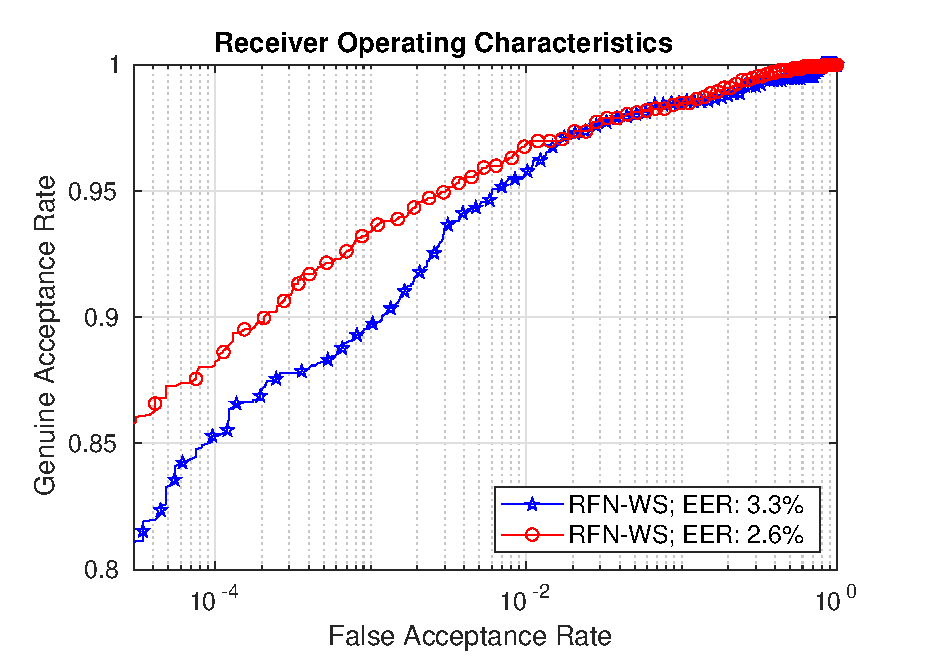
\includegraphics[width=\linewidth]{Figures/update-fkv3/fkv3-roc_compare_new.eps}
        \caption{Compare performance on the Finger Knuckle V3 Dataset (with deformable) segmented by YOLOV5.}
	\end{subfigure}
    \begin{subfigure}[b]{0.8\linewidth}
		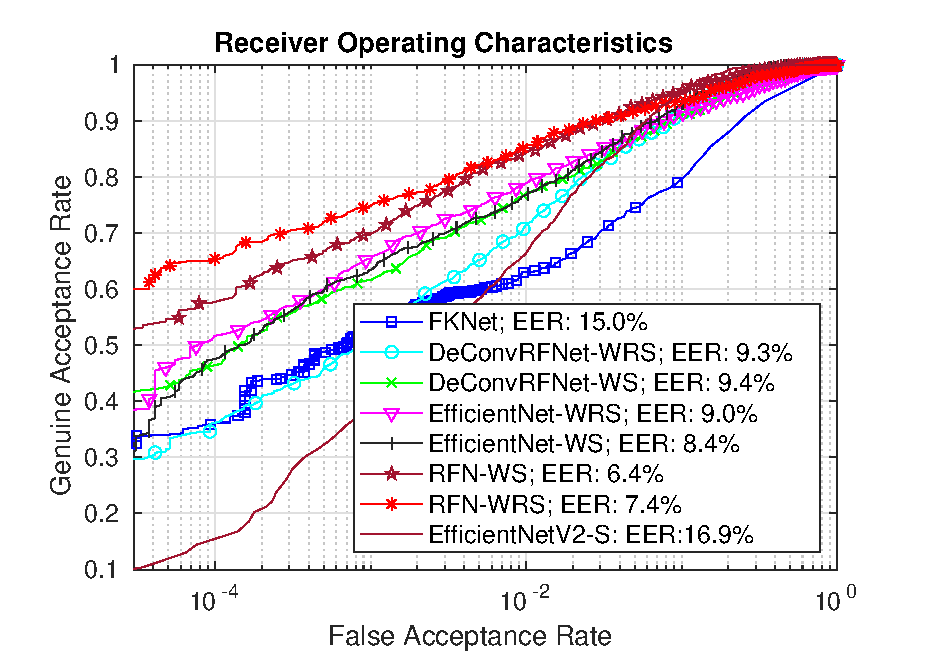
\includegraphics[width=\linewidth]{Figures/add-efficientv2-s/fkv3-roc_compare_new.eps}
        \caption{Compare performance on the Finger Knuckle V3 Dataset (with deformable) offered by database.}
	\end{subfigure}
	\begin{subfigure}[b]{0.8\linewidth}
		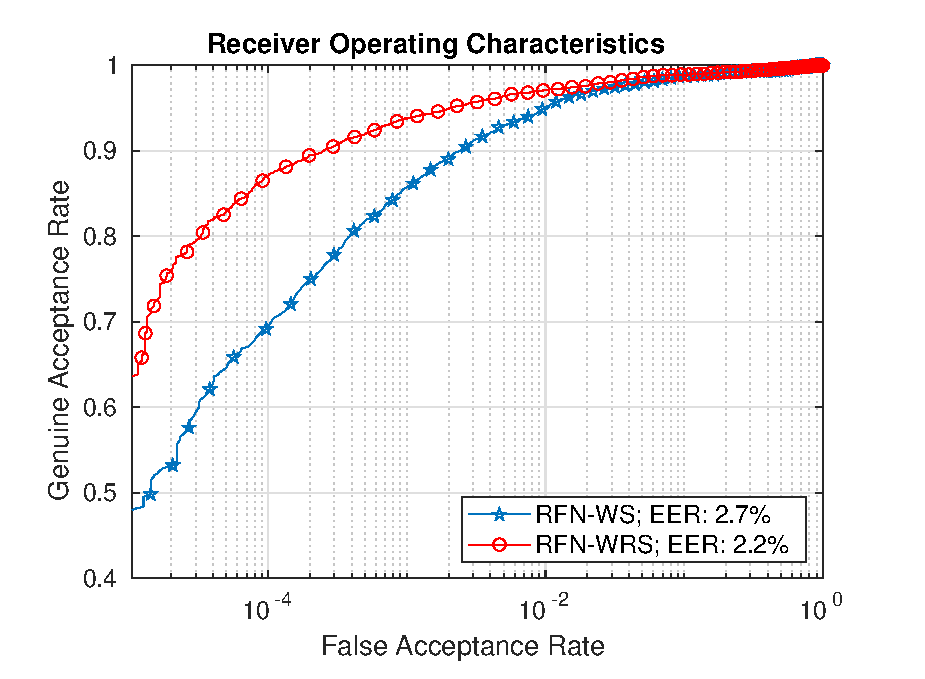
\includegraphics[width=\linewidth]{Figures/update-fkv3/cross-hd-roc_compare_new.eps}
        \caption{Cross database performance on the Index Finer Knuckle of Hand Dorsal Dataset by using the Figure (a) model results}
	\end{subfigure}
    \caption{}
    \label{update-fkv3}
\end{figure}

\textcolor{red}{From the Figure \ref{update-fkv3} (a) and (b), with the help of Yolov5, the quality of segmented finger Knuckle by Yolov5 is very high. Meanwhile, with the help of YOLOV5, the RFNet-WRS performance is slightly higher than local feature descriptors based on key points matching \cite{kumar2020contactless}.}